\chapter{Конструкторская часть}
В данном разделе представлены требования к программному обеспечению, рассмотрены структуры данных, алгоритмы и математические уравнения, выбранные для построения сцены.

\section{Требования к программному обеспечению}

Программное обеспечение должно обеспечивать следующую функциональность:

\begin{itemize}
    \item[$-$] Генерацию тел: шара, куба, параллелепипеда и шестигранной призмы, с возможностью задания их размеров, цветов и координат центра;
    \item[$-$] Моделирование клетчатой прямоугольной площадки с лунками, соответствующими указанным телам;
    \item[$-$] Реализацию процесса падения тел на площадку по запросу пользователя;
    \item[$-$] Определение попадания тела в соответствующую ей лунку, вывод соответствующих сообщений и удаление тела и лунки при успешном попадании;
    \item[$-$] Вывод сообщений при непопадании тела или попадании в чужую лунку и удаление тел из сцены;
    \item[$-$] Возможность изменения положения камеры для обзора сцены под разными углами и ракурсами;
    \item[$-$] Реализация источника света с возможностью задания его положения и интенсивности.
\end{itemize}

\section{Используемые структуры данных}

Для реализации работы программы разработаны следующие основные структуры данных:

\begin{enumerate}
    \item Сцена содержит:
    
    \begin{itemize}
        \item[$-$] Массив объектов сцены, включая модели, лунки и площадку;
        \item[$-$] Камеру и источник освещения;
        \item[$-$] Методы для добавления и удаления объектов со сцены.
    \end{itemize}
    
    \item Трехмерное тело включает в себя:
    
    \begin{itemize}
        \item[$-$] Массив вершин;
        \item[$-$] Массив граней, формирующих аппроксимацию поверхности;
        \item[$-$] Массив нормалей к вершинам для расчета освещения;
        \item[$-$] Цвет поверхности тела;
        \item[$-$] Положение и вращение тела в пространстве;
        \item[$-$] Матрицу преобразований для применения трансформаций к телу.
    \end{itemize}
    
    \item Вершина содержит:
    
    \begin{itemize}
        \item[$-$] Положение в пространстве;
        \item[$-$] Нормаль в данной вершине.
    \end{itemize}
    
    \item Грань модели содержит:
    
    \begin{itemize}
        \item[$-$] Индексы вершин A, B, C в списке вершин модели, образующих грань.
    \end{itemize}
    
    \item Камера содержит:
    
    \begin{itemize}
        \item[$-$] Положение в пространстве;
        \item[$-$] Направление взгляда;
        \item[$-$] Методы для изменения положения и ориентации камеры. 
    \end{itemize}
    
    \item Источник освещения содержит:
    
    \begin{itemize}
        \item[$-$] Положение в пространстве;
        \item[$-$] Интенсивность света.
    \end{itemize}
    
    \item Для представления тел и соответствующих им лунок необходима дополнительная информация:
    
    \begin{itemize}
        \item[$-$] Тип тела или лунки;
        \item[$-$] Размер и другие параметры, специфичные для конкретного тела.
    \end{itemize}
\end{enumerate}
\section{Алгоритм построения изображения}

Алгоритм генерации изображения представлен в виде диаграммы, оформленной в соответствии с нотацией IDEF0 и отражающей общую декомпозицию алгоритма [6].
\begin{figure}[h]
	\centering
	\includesvg[scale=0.7]{img/01_A-0.svg}
	\caption{Функциональная схема алгоритма построения изображения, декомпозиция верхнего уровня}
	\label{fig:classic}
\end{figure}
\begin{figure}[h]
	\centering
	\includesvg[scale=0.7]{img/02_A0.svg}
	\caption{Функциональная схема алгоритма построения изображения, декомпозиция уровня А0}
	\label{fig:classic}
\end{figure}
\begin{figure}[h]
	\centering
    \includesvg[scale=0.7]{img/03_A1.svg}
	% 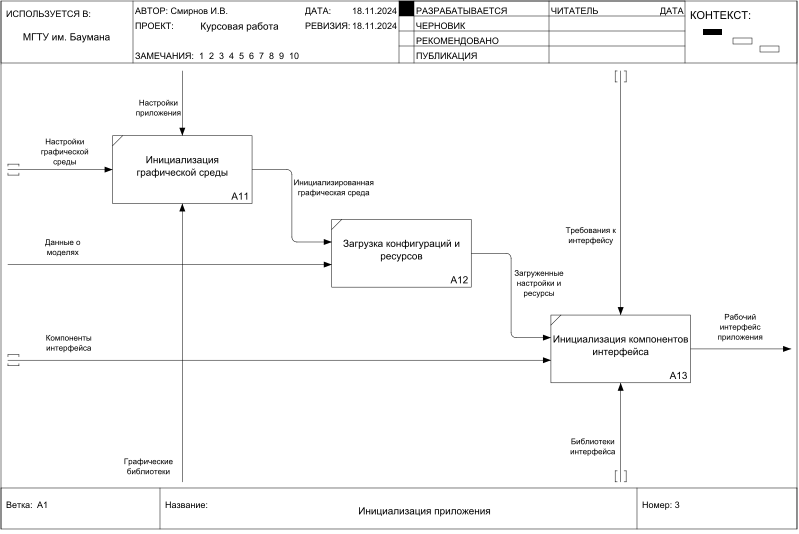
\includegraphics[scale=0.5]{img/03_A1.png}
	\caption{Функциональная схема алгоритма построения изображения, декомпозиция уровня А1}
	\label{fig:classic}
\end{figure}
\begin{figure}[h]
	\centering
    \includesvg[scale=0.7]{img/04_A2.svg}
	% 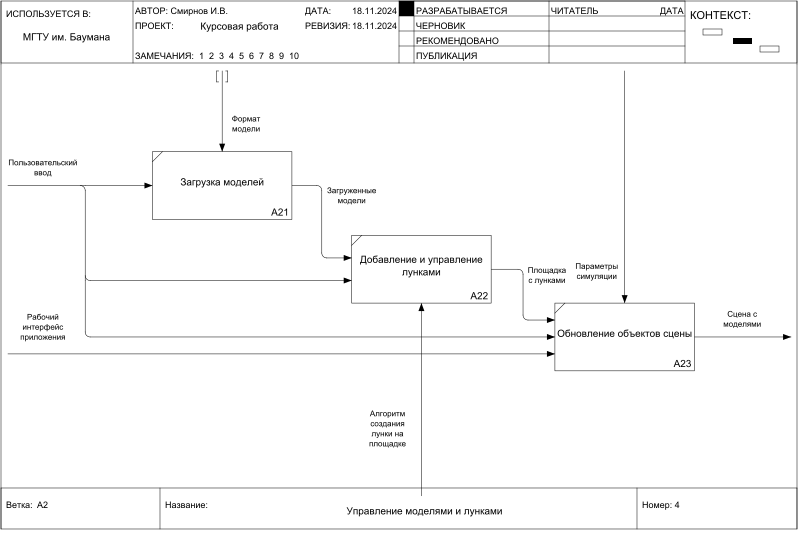
\includegraphics[scale=0.5]{img/04_A2.png}
	\caption{Функциональная схема алгоритма построения изображения, декомпозиция уровня А2}
	\label{fig:classic}
\end{figure}
\begin{figure}[h]
	\centering
    \includesvg[scale=0.7]{img/05_A3.svg}
	% 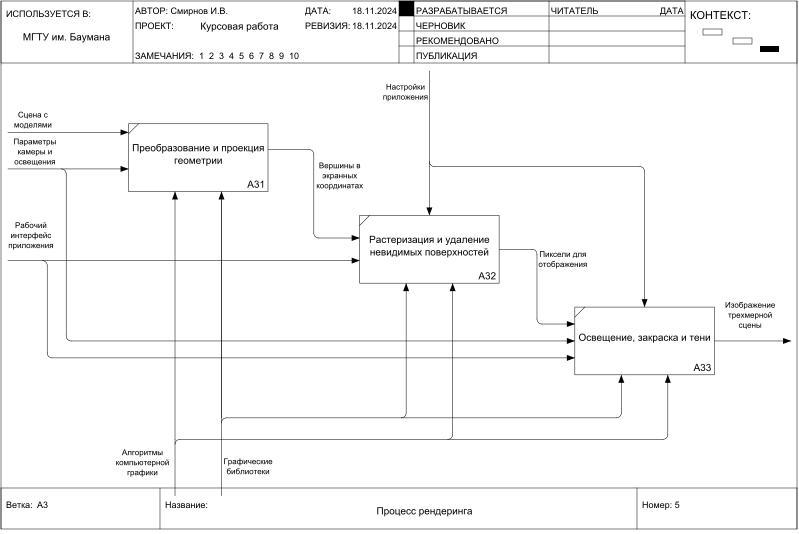
\includegraphics[scale=0.5]{img/05_A3.png}
	\caption{Функциональная схема алгоритма построения изображения, декомпозиция уровня А3}
	\label{fig:classic}
\end{figure}
\clearpage

\section{Перевод координат в экранные}

Для преобразования координат из мирового пространства в экранное используется следующая последовательность шагов. Сначала применяется матрица модели, включающая трансформации объекта, такие как повороты, масштабирование и перемещения. Затем применяется видовая матрица, определяющая положение и ориентацию камеры. Видовая матрица вычисляется как:
\begin{equation}
    \label{for}
    M_\textup{вид} = M_\textup{пер} \cdot M_\textup{пов},
\end{equation}
где $M_\textup{пер}$ отвечает за перенос точки камеры в начало координат, а $M_\textup{пов}$ выравнивает оси камеры. После этого применяется проекционная матрица, которая используется для перехода от трехмерных координат к двумерным. Для перспективной проекции используется следующая матрица:
\begin{equation}
    \label{for}
    M_\textup{проэк} = \begin{bmatrix}
    \frac{1}{tg(fov/2) \cdot aspect} & 0 & 0 & 0 \\
    0 & \frac{1}{tg(fov/2)} & 0 & 0 \\
    0 & 0 & \frac{far}{far - near} & 1 \\
    0 & 0 & -\frac{far \cdot near}{far - near} & 0
    \end{bmatrix},
\end{equation}
где $fov$ $-$ угол обзора, $aspect$ $-$ соотношение сторон экрана, и $far, near$ $-$ расстояния до ближней и дальней плоскостей отсечения. Наконец, применяется матрица viewport, преобразующая координаты в экранные. Она задается как:
\begin{equation}
    \label{for}
    M_{viewport} = \begin{bmatrix}
    \frac{W}{2} & 0 & 0 & \frac{W}{2} \\
    0 & -\frac{H}{2} & 0 & \frac{H}{2} \\
    0 & 0 & 1 & 0 \\
    0 & 0 & 0 & 1
    \end{bmatrix},
\end{equation}
где $W, H$ $-$ ширина и высота экрана в пикселях. После применения всех матриц конечные координаты преобразуются в экранные.

\section{Алгоритм, использующий Z-буфер}

Алгоритм Z-буфера применяется для удаления невидимых поверхностей. На первом этапе Z-буфер инициализируется максимальными значениями глубины:
\begin{equation}
    \label{for}
    z_{buffer}[x][y] = z_{max}.
\end{equation}
Далее, для каждого треугольника сцены его вершины проецируются в экранное пространство, и треугольник растеризуется по пикселям. Для каждого пикселя вычисляется глубина текущего треугольника по формуле:
\begin{equation}
    \label{for}
    z = \frac{Ax + By + C}{D},
\end{equation}
где $A, B, C, D$ $-$ коэффициенты плоскости треугольника. Если глубина пикселя меньше значения в Z-буфере, то значение Z-буфера и цвета пикселя обновляется:
\begin{equation}
    \label{for}
    z_{buffer}[x][y] = z, \quad color[x][y] = color_{t}.
\end{equation}
% Схема алгоритма представлена на рисунке \ref{fig}.

% \begin{figure}[h]
%     \centering
%     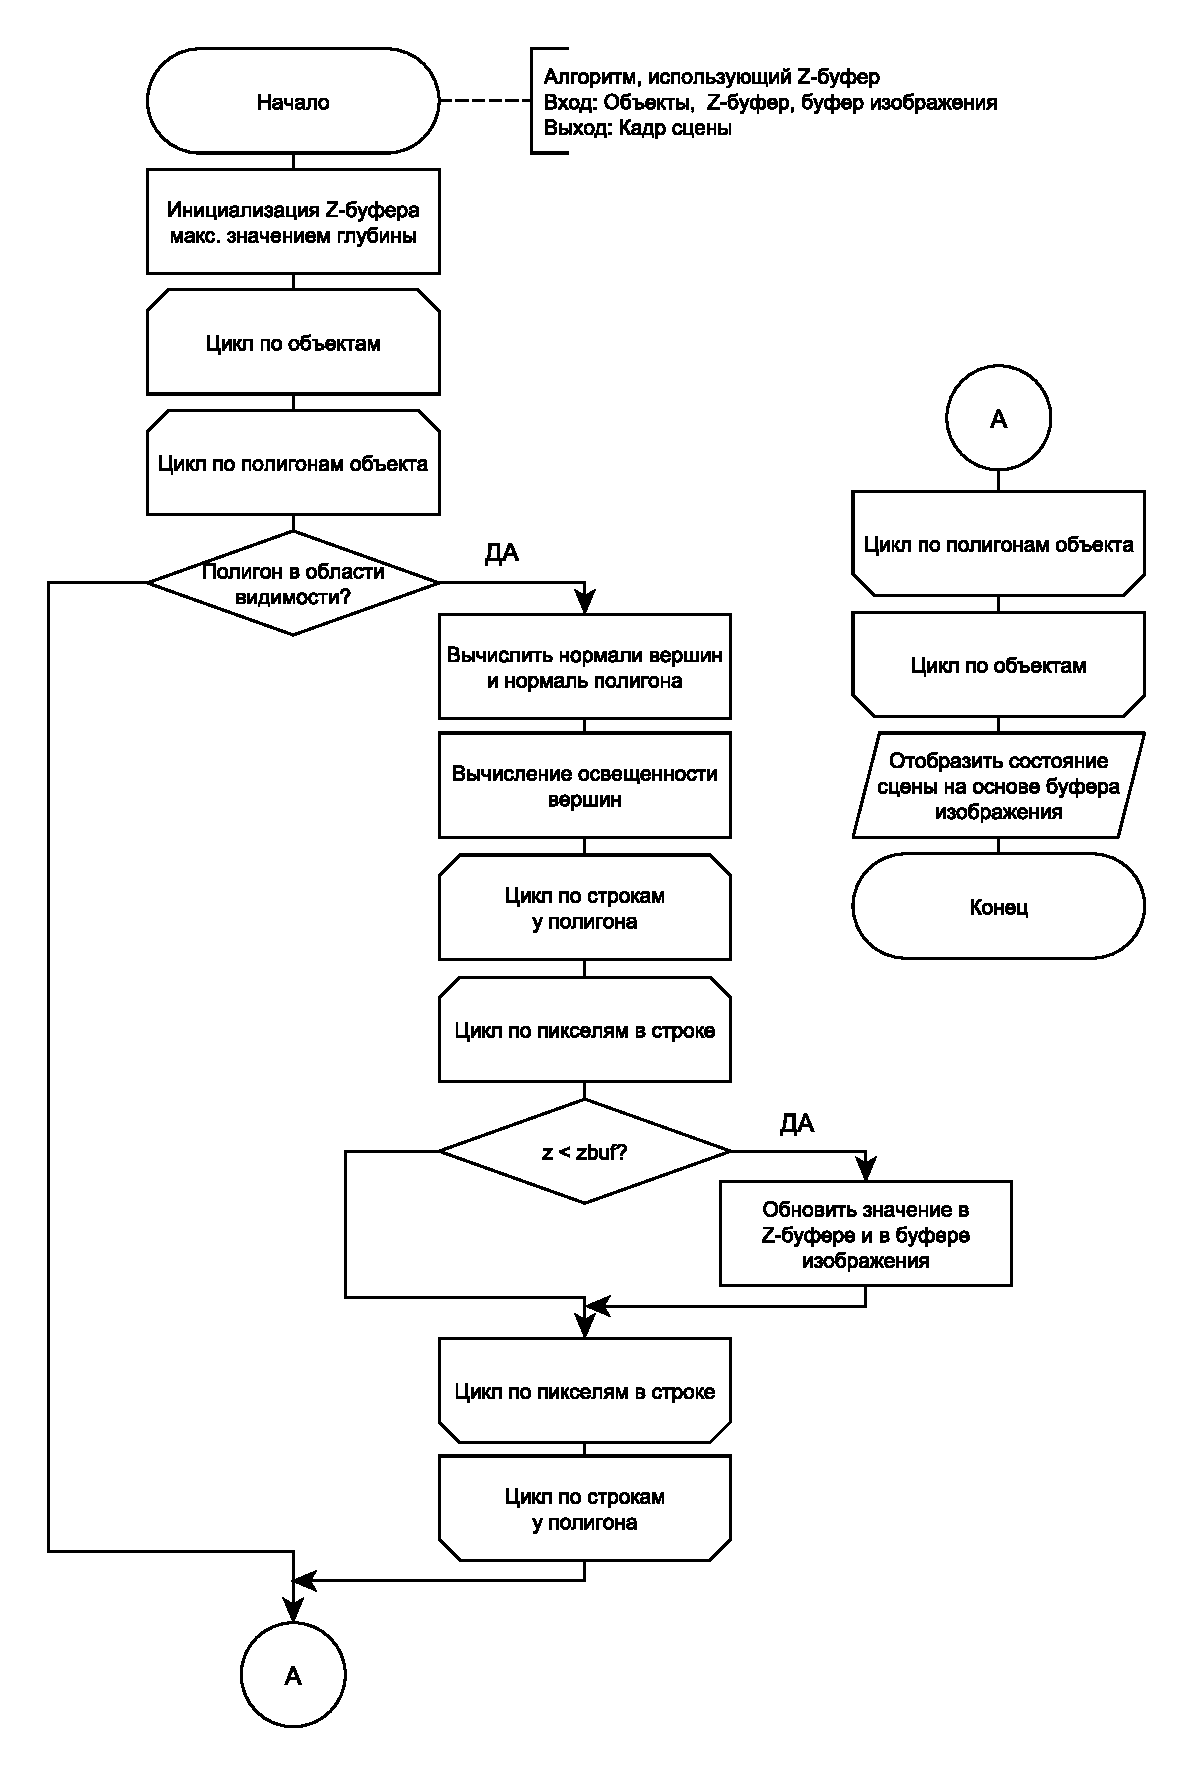
\includegraphics[scale=0.6]{img/zbuf.eps}
%     \caption{Схема алгоритма, использующего Z-буфер}
%     \label{fig}
% \end{figure}
% \clearpage
\section{Алгоритм моделирования лунок}

Лунки моделируются путем изменения высоты и нормалей вершин сетки площадки. Для каждой лунки определяются ее тип, координаты центра в сетке $(x_0, z_0)$ и размеры. Для сферических лунок смещение по оси $y$ вычисляется по уравнению сферы:
\begin{equation}
    \label{for}
    y = -\sqrt{r^2 - (x - x_0)^2 - (z - z_0)^2},
\end{equation}
где $(x, z)$ $-$ координаты выбранной области сетки площадки для лунки, $r$ $-$ радиус лунки. Для остальных типов лунок смещение по $y$ всегда фиксированное и вычисляется как:
\begin{equation}
    \label{for}
    y = -a,
\end{equation}
где $a$ $-$ глубина лунки.

После определения новых высот для вершин внутри лунки, для шестигранных и цилиндрических лунок по границе области формируются вертикальные стенки. Алгоритм следующий:
\begin{enumerate}
    \item Определяется периметр лунки: набор вершин, где лунка переходит из углубления в исходный уровень.
    \item Для каждой пары соседних вершин на периметре (например, $(v_{\text{1}}, v_{\text{2}})$) создаются дополнительные вершины, смещенные вниз на глубину лунки, формируя четыре точки: верхние точки периметра $(v_{\text{1}}, v_{\text{2}})$ с $y=0$, и соответствующие им нижние точки $(v_{\text{3}}, v_{\text{4}})$ с $y = -a$.
    \item С помощью этих четырех точек формируется две треугольные грани (два треугольника), образуя вертикальную стенку.
\end{enumerate}

Для шестиугольных и цилиндрических лунок стены немного смещаются наружу от центра лунки на малую величину $e$:
\begin{equation}
    (x', z') = (x + e \cdot \frac{dx}{\sqrt{dx^2+dz^2}}, z + e \cdot \frac{dz}{\sqrt{dx^2+dz^2}}),
\end{equation}
где $dx = x - x_0$, $dz = z - z_0$. Это позволяет визуально отделить стенки лунки от основной поверхности.
% \section{Перевод координат в экранные}

% Для преобразования координат из мирового пространства в экранное используется следующая последовательность шагов:

% \begin{enumerate}
%     \item Применение мировой матрицы, включающей трансформации объекта (повороты, масштабирование и перемещения).
%     \item Применение видовой матрицы, определяющей положение и ориентацию камеры. Видовая матрица вычисляется как:
%     \begin{equation}
%         \label{for}
%         M_\textup{вид} = M_\textup{пер} \cdot M_\textup{пов},
%     \end{equation}
%     где $M_\textup{пер}$ отвечает за перенос точки камеры в начало координат, а $M_\textup{пов}$ выравнивает оси камеры.
%     \item Применение проекционной матрицы, которая используется для перехода от трехмерных координат к двумерным. Для перспективной проекции используется следующая матрица:
%     \begin{equation}
%         \label{for}
%         M_\textup{проэк} = \begin{bmatrix}
%         \frac{1}{tg(fov/2) \cdot aspect} & 0 & 0 & 0 \\
%         0 & \frac{1}{tg(fov/2)} & 0 & 0 \\
%         0 & 0 & \frac{far}{far - near} & 1 \\
%         0 & 0 & -\frac{far \cdot near}{far - near} & 0
%         \end{bmatrix},
%     \end{equation}
%     где $fov$ $-$ угол обзора, $aspect$ $-$ соотношение сторон экрана, и $far, near$ $-$ расстояния до ближней и дальней плоскостей отсечения.
%     \item Применение матрицы viewport, преобразующей координаты в экранные. Она задается как:
%     \begin{equation}
%         \label{for}
%         M_{viewport} = \begin{bmatrix}
%         \frac{W}{2} & 0 & 0 & \frac{W}{2} \\
%         0 & -\frac{H}{2} & 0 & \frac{H}{2} \\
%         0 & 0 & 1 & 0 \\
%         0 & 0 & 0 & 1
%         \end{bmatrix},
%     \end{equation}
%     где $W, H$ $-$ ширина и высота экрана в пикселях.
% \end{enumerate}

% После применения всех матриц конечные координаты преобразуются в экранные.

% \section{Алгоритм, использующий Z-буфер}

% Алгоритм Z-буфера применяется для удаления невидимых поверхностей. Основные шаги:

% \begin{enumerate}
%     \item Инициализация Z-буфера максимальными значениями глубины:
%     \begin{equation}
%         \label{for}
%         z_{buffer}[x][y] = \infty.
%     \end{equation}
%     \item Для каждого треугольника сцены:
%     \begin{itemize}
%     \item Проекция его вершин в экранное пространство.
%     \item Растеризация треугольника по пикселям.
%     \item Для каждого пикселя вычисление глубины  текущего треугольника:
%         \begin{equation}
%             \label{for}
%             z = \frac{Ax + By + C}{D},
%         \end{equation}
%     где $A, B, C, D$ $-$ коэффициенты плоскости треугольника.
%     \item Если глубина пикселя меньше значения в Z-буфере, то значение Z-буфера и цвета пикселя обновляется:
%         \begin{equation}
%             \label{for}
%             z_{buffer}[x][y] = z, \quad color[x][y] = color_{t}.
%         \end{equation}
%     \end{itemize}
% \end{enumerate}

% Схема алгоритма представлена на рисунке \ref{fig}.

% \begin{figure}[h]
%     \centering
%     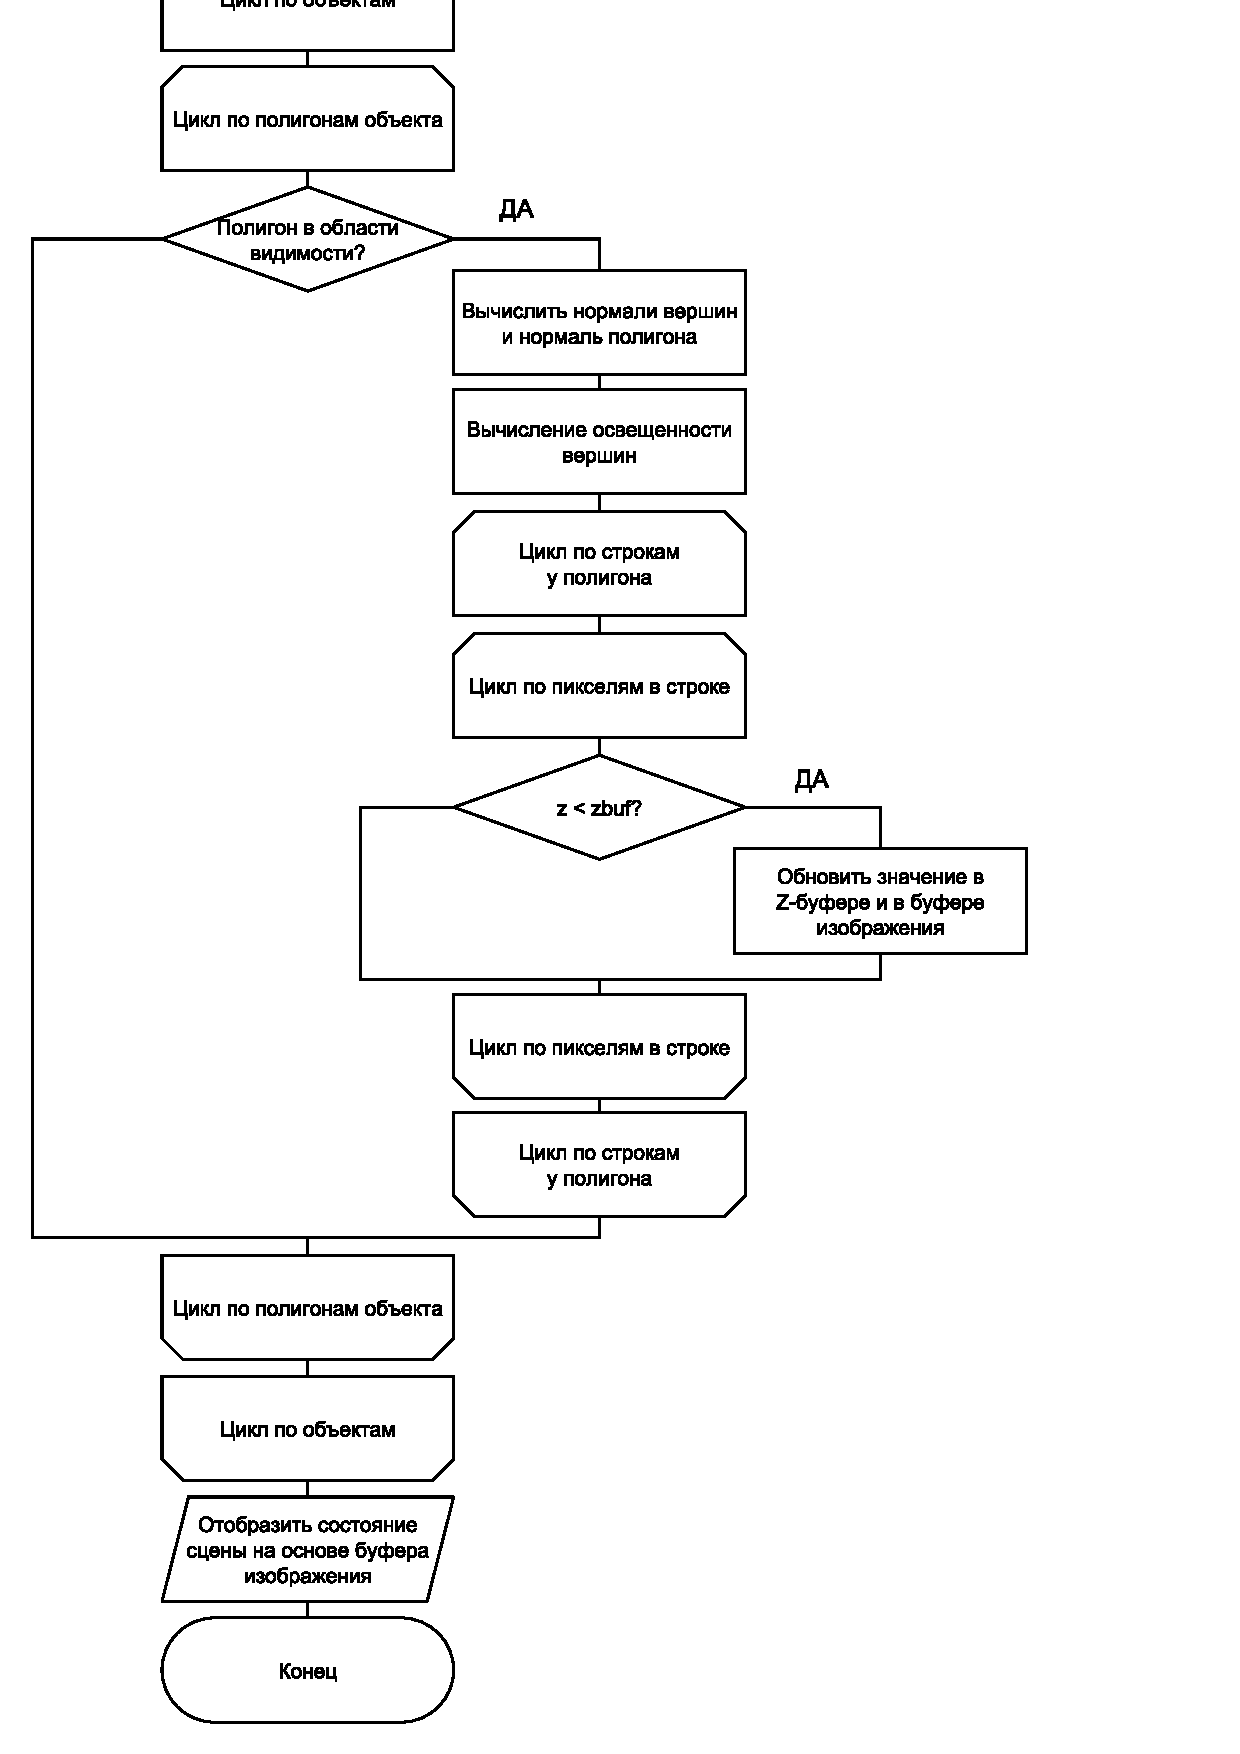
\includegraphics[scale=0.8]{img/zbuf.png}
%     \caption{Схема алгоритма, использующего Z-буфер}
%     \label{fig}
% \end{figure}

% \section{Алгоритм создания лунок}

% Лунки создаются путем изменения высоты и нормалей вершин сетки площадки. Основные шаги:

% \begin{enumerate}
%     \item Для каждой лунки определяются ее тип (сферическая или кубическая), координаты в сетке $(x_0, z_0)$ и размеры.
%     \item Для сферических лунок вычисляется смещение по оси  по уравнению сферы:
%         \begin{equation}
%             \label{for}
%             y = -\sqrt{r^2 - (x - x_0)^2 - (z - z_0)^2},
%         \end{equation}
%     где $(x, z)$ $-$ координаты выбранной области сетки площадки для лунки, $((x-x_0), 0, (z-z_0))$ $-$ центр лунки, $r$ $-$ радиус.
%     \item Для кубических лунок смещение по  фиксированное на глубину лунки:
%         \begin{equation}
%             \label{for}
%             y = -a,
%         \end{equation}
%         где $a$ $-$ сторона куба.
%     \item Для каждой вершины обновляются нормали: для сферических лунок нормаль рассчитывается как вектор от центра лунки к точке, а для кубических нормаль остается вертикальной.
% \end{enumerate}

\section{Вычисление нормалей}

Нормали необходимы для освещения и корректного отображения поверхностей. Сначала для всех вершин нормали инициализируются нулевым вектором. Для каждого треугольника вычисляется нормаль грани по следующей формуле:
\begin{equation}
    \vec{N} = \frac{(\vec{V}_2 - \vec{V}_1) \times (\vec{V}_3 - \vec{V}_1)}{|(\vec{V}_2 - \vec{V}_1) \times (\vec{V}_3 - \vec{V}_1)|},
\end{equation}
где $\vec{V}_1$, $\vec{V}_2$, $\vec{V}_3$ $-$ вершины треугольника. Вычисленная нормаль добавляется к нормалям ее вершин. Затем нормали всех вершин нормализуются:
\begin{equation}
    \vec{N}_v = \frac{\vec{N}}{|\vec{N}|},
\end{equation}
где $\vec{N}_v$ $-$ суммарный вектор нормали вершины.

\section{Освещение}

В программе используется всенаправленный источник света, расположенный в заданной точке пространства. Он испускает свет во всех направлениях, а освещение рассчитывается по модели Ламберта.

Для каждой вершины вычисляется итоговая освещенность $I$ как сумма фонового и диффузного освещения:
\begin{equation}
I = I_{a} + I_{d},
\end{equation}
где $I_{a}$ $-$ фоновая составляющая (фиксированная величина), а $I_{d}$ $-$ диффузное освещение, рассчитываемое по формуле:
\begin{equation}
I_{d} = \max(0, \vec{N} \cdot \vec{L}).
\end{equation}

Здесь $\vec{N}$ $-$ нормаль вершины, а $\vec{L}$ $-$ нормализованный вектор направления от вершины к источнику света. Значение $\max(0, \vec{N} \cdot \vec{L})$ исключает отрицательные значения, которые могут возникнуть, если нормаль и направление света образуют тупой угол.

Результирующая освещенность каждой вершины интерполируется по граням треугольников, что позволяет плавно переходить между яркими и темными областями объекта.


% \section{Представление алгоритмов}

% На вход алгоритмов подаются две матрицы: $M_{1}$ размера $M \times N$, $M_{2}$ размера $N \times K$, где $M, N, K$ $-$ неотрицательные целые числа; на выходе - матрица $M_{3}$ размера $M \times K$.

% На рисунках \ref{fig:classic} $-$ \ref{fig:vinograd_opt} приведены схемы трех алгоритмов умножения матриц: классического, Винограда, оптимизированного Винограда.

% \clearpage

% \begin{figure}[h]
% 	\centering
% 	\includegraphics[scale=0.8]{img/classic.eps}
% 	\caption{Схема классического алгоритма умножения матриц}
% 	\label{fig:classic}
% \end{figure}

\vspace{5mm}
\textbf{ВЫВОД}

В данном разделе были представлены требования к программному обеспечению, рассмотрены структуры данных, алгоритмы и математические уравнения, выбранные для построения сцены.

\clearpage